\section{UNO-1 Grafo (p=1)}

\hspace*{3em} Quando o número de jogadores é \( p = 1 \), uma carta \( t' \) corresponde a \( t \) se, e somente se, \( t \) corresponde a \( t' \). Isso torna a relação de “correspondência” simétrica, e o grafo UNO-1 pode ser visto como não direcionado. 

\subsection{Detalhamento}

\hspace*{3em} Para entender melhor, considere as seguintes definições e propriedades:

\begin{itemize}
    \item \textbf{Carta:} Uma carta \( t \) é um elemento do conjunto de cartas disponíveis no jogo UNO.
    \item \textbf{Correspondência:} Dizemos que uma carta \( t' \) corresponde a uma carta \( t \) se elas podem ser jogadas uma após a outra de acordo com as regras do jogo.
    \item \textbf{Simetria:} A relação de correspondência é simétrica, ou seja, se \( t' \) corresponde a \( t \), então \( t \) também corresponde a \( t' \).
    \item \textbf{Grafo UNO-1:} Um grafo onde os vértices representam as cartas e as arestas representam a relação de correspondência entre as cartas.
\end{itemize}

\subsection{Propriedades do Grafo UNO-1}

\begin{itemize}
    \item \textbf{Não direcionado:} Devido à simetria da relação de correspondência, o grafo UNO-1 é não direcionado. Isso significa que se existe uma aresta entre \( t \) e \( t' \), então também existe uma aresta entre \( t' \) e \( t \).
    \item \textbf{Conectividade:} O grafo pode ser analisado em termos de componentes conectados, onde cada componente representa um conjunto de cartas que podem ser jogadas em sequência.
\end{itemize}

\subsection{Exemplo}
\hspace*{3em} Considere o seguinte exemplo de jogo de UNO de apenas uma pessoa, com \( C = \{(1, 3), (2, 2), (2, 3), (2, 3), (2, 4), (3, 2), (3, 4), \\ (4, 1), (4, 3)\} \)


\begin{center}
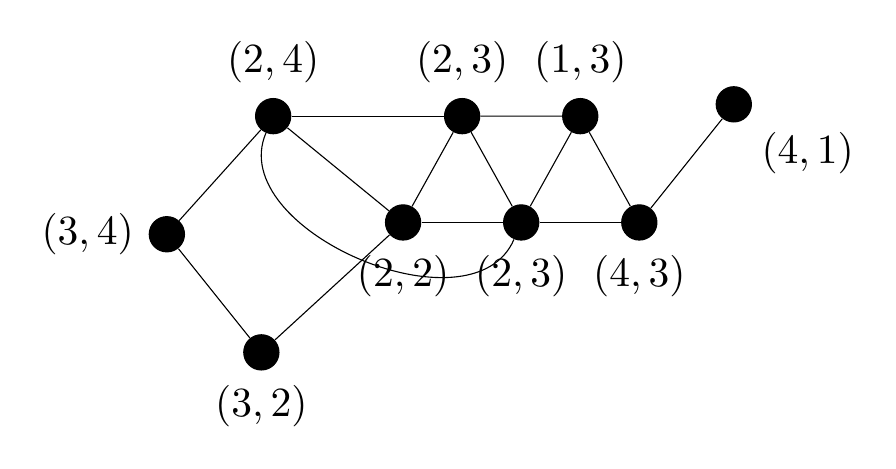
\begin{tikzpicture}[scale=1.5, transform shape]
    \node[draw, circle, fill=black, inner sep=3pt, label=left:{$(3, 4)$}] (G) at (0, 0) {};
    \node[draw, circle, fill=black, inner sep=3pt, label=above:{$(2, 4)$}] (E) at (0.9, 1) {};
    \node[draw, circle, fill=black, inner sep=3pt, label=below:{$(3, 2)$}] (F) at (0.8,-1) {};
    \node[draw, circle, fill=black, inner sep=3pt, label=below:{$(2, 2)$}] (B) at (2,0.1) {};
    \node[draw, circle, fill=black, inner sep=3pt, label=below:{$(4, 3)$}] (I) at (4,0.1) {};
    \node[draw, circle, fill=black, inner sep=3pt, label=above:{$(2, 3)$}] (D) at (2.5,1) {};
    \node[draw, circle, fill=black, inner sep=3pt, label=above:{$(1, 3)$}] (A) at (3.5,1) {};
    \node[draw, circle, fill=black, inner sep=3pt, label=below:{$(2, 3)$}] (C) at (3,0.1) {};
    \node[draw, circle, fill=black, inner sep=3pt, label=below right:{$(4, 1)$}] (H) at (4.8,1.1) {};

    \draw (G) -- (E);
    \draw (G) -- (F);
    \draw (E) -- (B);
    \draw (F) -- (B);
    \draw (C) -- (B);
    \draw (C) -- (I);
    \draw (H) -- (I);
    \draw (A) -- (I);
    \draw (A) -- (C);
    \draw (D) -- (C);
    \draw (D) -- (B);
    \draw (D) -- (A);
    \draw (E) -- (D);
    \draw[bend right=90] (E) to (C);

\end{tikzpicture}
\end{center}

\textbf{\color{red} {AINDA FALTA ARESTAS}}

\hspace*{2em} Aqui investigamos algumas propriedades básicas dos grafos UNO-1. Em grafos UNO-1, todos os vértices cujas cartas correspondentes possuem a mesma cor ou o mesmo número formam uma clique\footnote{Uma clique em um grafo é um subconjunto de seus vértices tal que todos os vértices do subconjunto são adjacentes entre si. Em outras palavras, é um grafo completo induzido pelo subconjunto de vértices.}, em outra palavras, todos os vértices de mesma cor ou número estão conectados.


\hspace*{2em} O grafo de linha \( L(G) \) de um grafo dado \( G \) é o grafo cujos vértices são as arestas de \( G \), e \(\{e,e'\} \in E(L(G))\) para \( e,e' \in V(L(G)) = E(G) \) se e somente se \( e \) e \( e' \) compartilham um vértice em \( G \).

\begin{center}
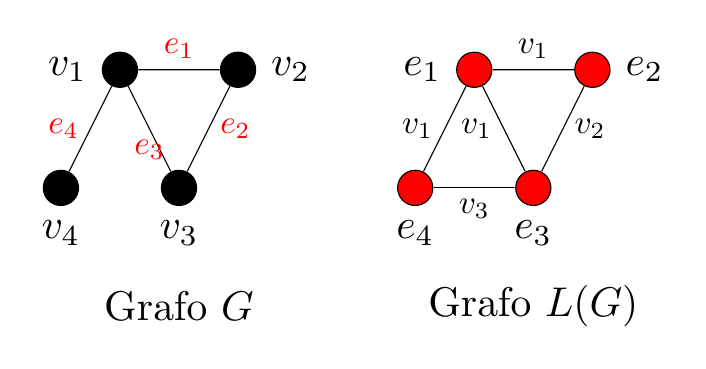
\begin{tikzpicture}[scale=1.5, transform shape]
    % Grafo G
    \node[draw, circle, fill=black, inner sep=3pt, label=left:{$v_1$}] (v1) at (0, 1) {};
    \node[draw, circle, fill=black, inner sep=3pt, label=right:{$v_2$}] (v2) at (1, 1) {};
    \node[draw, circle, fill=black, inner sep=3pt, label=below:{$v_3$}] (v3) at (0.5, 0) {};
    \node[draw, circle, fill=black, inner sep=3pt, label=below:{$v_4$}] (v4) at (-0.5, 0) {};
    \draw (v1) -- node[above, scale=0.8, text=red] {$e_1$} (v2);
    \draw (v2) -- node[right, scale=0.8, text=red] {$e_2$} (v3);
    \draw (v3) -- node[below, scale=0.8, text=red] {$e_3$} (v1);
    \draw (v4) -- node[left, scale=0.8, text=red] {$e_4$} (v1);

    \node at (0.5, -1) {Grafo \(G\)};

    % Grafo L(G)
    \node[draw, circle, fill=red, inner sep=3pt, label=left:{$e_1$}] (e1) at (3, 1) {};
    \node[draw, circle, fill=red, inner sep=3pt, label=right:{$e_2$}] (e2) at (4, 1) {};
    \node[draw, circle, fill=red, inner sep=3pt, label=below:{$e_3$}] (e3) at (3.5, 0) {};
    \node[draw, circle, fill=red, inner sep=3pt, label=below:{$e_4$}] (e4) at (2.5, 0) {};
    \draw (e1) -- node[above, scale=0.8, text=black] {$v_1$} (e2);
    \draw (e1) -- node[left, scale=0.8, text=black] {$v_1$} (e3);
    \draw (e1) -- node[left, scale=0.8, text=black] {$v_1$} (e4);
    \draw (e2) -- node[right, scale=0.8, text=black] {$v_2$} (e3);
    \draw (e3) -- node[below, scale=0.8, text=black] {$v_3$} (e4);

    \node at (3.5, -1) {Grafo \(L(G)\)};
\end{tikzpicture}
\end{center}

foi colocado rótulos para facilitar a visualização, mas não é necessários para a definição do grafo.

\textbf{\color{red} entender melhor o paragrafo anterior e o seguinte, dez da noite ta foda}

\hspace*{2em} Como uma carta de UNO é um par ordenado de uma cor e um número, as cartas de UNO correspondem ao conjunto de arestas de um grafo bipartido, cujos conjuntos partites são cores e números. Assim, um grafo UNO-1 representa a adjacência de arestas (correspondentes às cartas) de um grafo bipartido. Esses argumentos levam ao seguinte fato.

\begin{tcolorbox}[colback=white, colframe=black!70, title=Lema 1]
Se \( G \) é um grafo bipartido, então \( L(G) \) é um grafo de linha.
\end{tcolorbox}

\begin{tcolorbox}[colback=white, colframe=black!70, title=Prova do Lema 1]
\begin{proof}
Seja \( G = (V, E) \) um grafo bipartido com partições \( V_1 \) e \( V_2 \). O grafo de linha \( L(G) \) é definido como o grafo cujos vértices são as arestas de \( G \) e duas arestas em \( L(G) \) são adjacentes se e somente se compartilham um vértice em \( G \).

Como \( G \) é bipartido, cada aresta \( e \in E \) conecta um vértice de \( V_1 \) a um vértice de \( V_2 \). Portanto, duas arestas \( e_1 \) e \( e_2 \) em \( G \) compartilham um vértice se e somente se uma extremidade de \( e_1 \) está em \( V_1 \) e a outra extremidade está em \( V_2 \), e o mesmo vale para \( e_2 \).

Assim, \( L(G) \) é um grafo onde os vértices representam as arestas de \( G \) e duas arestas são adjacentes se compartilham um vértice em \( G \). Portanto, \( L(G) \) é um grafo de linha.
\end{proof}
\end{tcolorbox}

\begin{tcolorbox}[colback=white, colframe=black!70, title=Corolário 1]
\begin{corollary}
Se \( G \) é um grafo bipartido, então o problema do Caminho Hamiltoniano em \( L(G) \) é NP-completo.
\end{corollary}
\end{tcolorbox}

\begin{tcolorbox}[colback=white, colframe=black!70, title=Prova do Corolário 1]
\begin{proof}
Segue diretamente do Teorema 1, que afirma que o problema do Caminho Hamiltoniano para grafos de linha de grafos bipartidos é NP-completo.
\end{proof}
\end{tcolorbox}


\begin{tcolorbox}[colback=white, colframe=black!70, title=Teorema 1]
O problema do Caminho Hamiltoniano para grafos de linha de grafos bipartidos é NP-completo.
\end{tcolorbox}

Portanto, como corolário deste teorema, vemos que UNO é um problema difícil mesmo para um único jogador.

\begin{tcolorbox}[colback=white, colframe=black!70, title=Teorema 2]
Uno-1 é NP-completo.
\end{tcolorbox}
\textbf{\color{red} MELHOR ESSA PROVA... PONTO IMPORTANTE DO TRABALHO}

\textbf{\color{red} {NÃO SEI SE VALE A PENA COLOCAR AS PROVAS EM ANEXOS}}

Para fins de completude, fornecemos uma prova direta e concisa do Teorema 2. Em contraste, a prova em \cite{FSU93} depende adicionalmente de \cite{B81}.

\begin{proof}[Demostração]
Um grafo cúbico é um grafo no qual todo vértice tem grau 3. Reduzimos do problema do Caminho Hamiltoniano para grafos cúbicos (HP-C), que é conhecido por ser NP-completo \cite{GJT76}.

Considere uma instância \( G \) de HP-C. Transformamos \( G \) em um grafo \( G' \), onde:
\[ V(G') = \{(x,e) \mid x \in V(G), e = \{x,y\} \in E(G)\} \]
\[ E(G') = \{((x,e),(y,e)) \mid e = \{x,y\} \in E(G)\} \cup \{((x,e_i),(x,e_j)) \mid e_i \neq e_j\} \]

Essa transformação divide qualquer vértice \( x \in V(G) \) em três novos vértices \( (x,e_1), (x,e_2), (x,e_3) \) para formar uma clique (triângulo), enquanto cada aresta \( e_i \) (i=1,2,3) incidente a \( x \) torna-se incidente a um novo vértice \( (x,e_i) \). A Figura 3 ilustra este "gadget" de nó.

\begin{center}
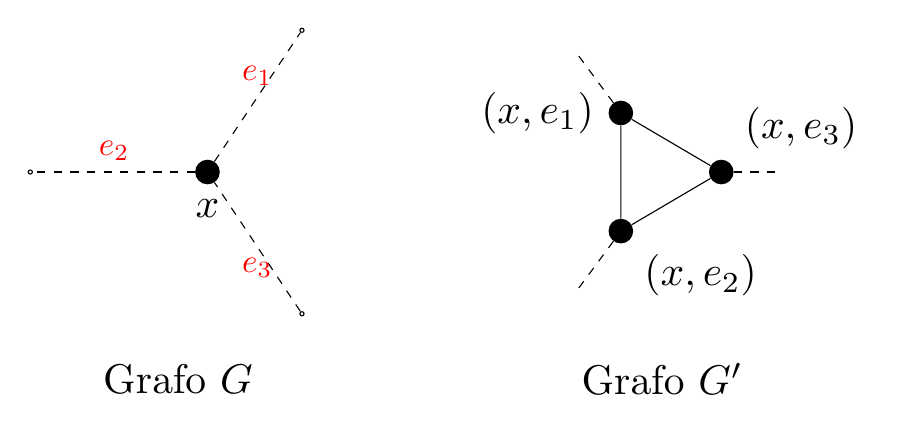
\begin{tikzpicture}[scale=1.5, transform shape]
    % Original graph G
    \node[draw, circle, fill=black, inner sep=2pt, label=below:{$x$}] (x) at (0, 0) {};
    \node[draw, circle, fill=white, inner sep=0.1pt] (y) at (0.8, 1.2) {};
    \node[draw, circle, fill=white, inner sep=0.1pt] (z) at (0.8, -1.2) {};
    \node[draw, circle, fill=white, inner sep=0.1pt] (v) at (-1.5, 0) {};
    \draw[dashed] (x) -- node[above, scale=0.8, text=red] {$e_1$} (y);
    \draw[dashed] (x) -- node[above, scale=0.8, text=red] {$e_2$} (v);
    \draw[dashed] (z) -- node[below, scale=0.8, text=red] {$e_3$} (x);

    \node at (-0.25, -1.75) {Grafo \(G\)};

        % Transformed graph G'
        \node[draw, circle, fill=black, inner sep=2pt, label=left:{$(x,e_1)$}] (xe1) at (3.5, 0.5) {};
        \node[draw, circle, fill=black, inner sep=2pt, label=above right:{$(x,e_3)$}] (xe3) at (4.35, 0) {};
        \node[draw, circle, fill=black, inner sep=2pt, label=below right:{$(x,e_2)$}] (xe2) at (3.5, -0.5) {};

        \draw (xe1) -- (xe2);
        \draw (xe2) -- (xe3);
        \draw (xe1) -- (xe3);

        \draw[dashed] (xe1) -- ++(-0.37, 0.5);
        \draw[dashed] (xe2) -- ++(-0.37, -0.5);
        \draw[dashed] (xe3) -- ++(0.5, 0);

    \node at (3.85, -1.75) {Grafo \(G'\)};
\end{tikzpicture}
\end{center}

Em seguida, preparamos o conjunto de cartas \( C \) do jogador de Uno-1 como o conjunto \( V(G') \), onde a cor e o número de \( (x,e) \) são \( x \) e \( e \), respectivamente. Podemos facilmente confirmar que existe uma aresta \( e = (t,t') \) em \( G' \) se e somente se \( t \) e \( t' \) correspondem. Assim, \( G' \) é o grafo UNO-1 correspondente ao conjunto de cartas \( C \).

Agora basta mostrar que existe um caminho Hamiltoniano em \( G \) se, e somente se, existe um caminho Hamiltoniano em \( G' \).
\end{proof}


\begin{figure}[hbt]
\centering
\scalebox{0.75}{\input{grafos/possible_tours.tps}}
\caption{Possible tours passing through a node gadget. 
Each dotted line is a part of a tour, 
and a square denotes either end of a tour. } 
\label{possible_tours}
\end{figure}

